\documentclass[12pt]{article}

\usepackage{setspace}
\usepackage{amsmath,amssymb}
\usepackage{graphicx}
\usepackage[pdftex,bookmarks=true,bookmarksopen=false,bookmarksnumbered=true,colorlinks=true,linkcolor=black]{hyperref}
\usepackage[utf8]{inputenc}
\usepackage{float}
\usepackage{pdfpages}
\usepackage[brazil]{babel}
\usepackage{helvet}
\usepackage{listings}
\usepackage{color}
\usepackage{graphicx}
 
\definecolor{dkgreen}{rgb}{0,0.6,0}
\definecolor{gray}{rgb}{0.5,0.5,0.5}
\definecolor{mauve}{rgb}{0.58,0,0.82}
\lstset{
  language=Python,                
  basicstyle=\footnotesize,           
  numbers=left,                   
  numberstyle=\tiny\color{gray},  
  stepnumber=2,                             
  numbersep=5pt,                  
  backgroundcolor=\color{white},    
  showspaces=false,               
  showstringspaces=false,         
  showtabs=false,                 
  frame=single,                   
  rulecolor=\color{black},        
  tabsize=2,                      
  captionpos=b,                   
  breaklines=true,                
  breakatwhitespace=false,        
  title=\lstname,                               
  keywordstyle=\color{blue},          
  commentstyle=\color{dkgreen},       
  stringstyle=\color{mauve},     
}

\renewcommand{\familydefault}{\sfdefault}

\newtheorem{theorem}{Theorem}[section]
\newtheorem{assumption}{Assumption}
\newtheorem{acknowledgment}{Acknowledgment}
\newtheorem{algorithm}{Algorithm}
\newtheorem{axiom}{Axiom}
\newtheorem{case}{Case}
\newtheorem{claim}{Claim}
\newtheorem{conclusion}{Conclusion} 
\newtheorem{condition}{Condition}
\newtheorem{conjecture}{Conjecture}
\newtheorem{corollary}{Corollary}[section]
\newtheorem{criterion}{Criterion}
\newtheorem{defn}{Definition}[section]

\newtheorem{example}{Example}[section]
\newtheorem{exercise}{Exercise}
\newtheorem{lemma}{Lemma}[section]
\newtheorem{notation}{Notation}
\newtheorem{problem}{Problem}
\newtheorem{proposition}{Proposition}[section]
\newtheorem{remark}{Remark}
\newtheorem{solution}{Solution}
\newtheorem{summary}{Summary}
\newenvironment{proof}[1][Proof]{\textbf{#1.} }{\rule{0.5em}{0.5em}}

\begin{document}

\begin{titlepage}
\begin{center}
\textbf{\LARGE Fundação Getulio Vargas}\\ 
\textbf{\LARGE Escola de Matemática Aplicada}\\
\textbf{\LARGE Curso de Graduação em Ciência de Dados}

\par
\vspace{170pt}
\textbf{\Large Regressão Logística}\\
\vspace{80pt}
\textbf{\Large Bianca Dias de Carvalho\\ Luis Fernando Laguardia}\\
\end{center}

\par
\vfill
\begin{center}
{{\normalsize Rio de Janeiro - Brasil}\\
{\normalsize \the\year}}
\end{center}
\end{titlepage}

\thispagestyle{empty}

\newpage
\begin{center}
\textbf{\LARGE Fundação Getulio Vargas}\\ 
\textbf{\LARGE Escola de Matemática Aplicada}\\
\textbf{\LARGE Curso de Graduação em Ciência de Dados}

\par
\vspace{100pt}
\textbf{\Large Regressão Logística}


\par
\vspace{150pt}

\end{center}

\par
\vspace{65pt}
\begin{center}


\hrulefill

\vspace{5pt}
\textbf{\Large Bianca Dias de Carvalho\\ Luis Fernando Laguardia}
\end{center}

\par
\vfill
\begin{center}
{{\normalsize Rio de Janeiro - Brasil}\\
{\normalsize \the\year}}
\end{center}

\thispagestyle{empty}

\newpage
\tableofcontents
\thispagestyle{empty}

\newpage
\section{Introdução}
\hspace{0.4cm} Este trabalho aborda a regressão logística, contendo notebooks em python, onde a regressão logística é aplicada em diversas bases de dados, com o fito de realizar previsões a partir de variáveis categóricas.

A regressão logística é uma técnica de mineração de dados, que consiste no processo de encontrar padrões e correlações em grandes conjuntos de dados para prever resultados, além disso, através dela também é possível obter a probabilidade de ocorrência de cada evento, assim como a influência de cada variável independente. 

A principal diferença entre a regressão logística e a regressão linear é que a variável dependente/resposta, atributo que se quer prever, é categórica, frequentemente binária. 

\newpage
\section{Desenvolvimento}
\hspace{0.4cm} Inicialmente, foi criado uma classe de regressão logística em python.
\\
\begin{lstlisting}
class LogisticRegression:
    def __init__(self, learning_rate=0.001, n_iters=1000):
        self.lr = learning_rate
        self.n_iters = n_iters
        self.weights = None
        self.bias = None

    def fit(self, X, y):
        n_samples, n_features = X.shape
        self.weights = np.zeros(n_features) #parametro inicial
        self.bias = 0 #parametro inicial

        #gradiente descendente
        for _ in range(self.n_iters):
            linear_model = np.dot(X, self.weights) + self.bias #aproxima y com a combinacao linear dos pesos e x somada a constante
            y_predicted = self._sigmoid(linear_model) #aplica a funcao sigmoide

            #computa os gradientes
            dw = (1 / n_samples) * np.dot(X.T, (y_predicted - y))
            db = (1 / n_samples) * np.sum(y_predicted - y)
            #atualiza os parametros
            self.weights -= self.lr * dw
            self.bias -= self.lr * db

    def predict(self, X):
        linear_model = np.dot(X, self.weights) + self.bias
        y_predicted = self._sigmoid(linear_model)
        y_predicted_cls = [1 if i > 0.5 else 0 for i in y_predicted]
        
        return np.array(y_predicted_cls)

    def _sigmoid(self, x):
        return 1 / (1 + np.exp(-x))
\end{lstlisting}

O gradiente descendente é um algoritmo de otimização, seu objetivo é minimizar algumas funções movendo-se iterativamente na direção de descida mais íngreme. O parâmetro \textit{learning rate} nos diz qual distância será percorrida em cada iteração, ele não pode ser muito pequeno devido ao custo computacional, nem muito grande por falhar em convergir no mínimo local. A função \textit{sigmoide} é aplicada à soma ponderada, essa função transforma varia de 0 a 1 e tem um formato S (não é linear) e basicamente tenta empurrar os valores de y para os extremos.
\\
\begin{lstlisting}
def plot(self, X, y, legend):
        # essa funcao plota o resultado apenas se X se referir a exatamente 2 variaveis
        if X.shape[1] != 2:
            raise ValueError("Can plot only for X's that refers to exactly 2 vars.")
        
        slope = -(self.weights[0]/self.weights[1])
        intercept = -(self.bias/self.weights[1])
        predictions = self.predict(X)

        sns.set_style('white')
        sns.scatterplot(x = X[:,0], y= X[:,1], hue=y.reshape(-1), style=predictions.reshape(-1));

        ax = plt.gca()
        ax.autoscale(False)
        x_vals = np.array(ax.get_xlim())
        y_vals = intercept + (slope * x_vals)
        plt.plot(x_vals, y_vals, c="k");
        
        plt.xlabel(legend[0])
        plt.ylabel(legend[1])
\end{lstlisting}

A função acima plota o resultado da regressão linear em um gráfico de dispersão onde nos eixos estão as variáveis independentes.

\vspace{100pt}

Após isso, as bases foram importadas e os dados foram normalizados. Como exemplo, será mostrado a importação e normalização de uma das bases.
\\
\begin{lstlisting}
df = pd.read_csv("db_estrelas.csv")

df = df[(df['Spectral Class'] == 'B') | (df['Spectral Class'] == 'M')]
df['Spectral Class'].replace(to_replace='B', value=1, inplace=True)
df['Spectral Class'].replace(to_replace='M', value=0, inplace=True)

# Seleção de Dados
dados = {
    'X' : ['Temperature (K)', 'Absolute magnitude(Mv)'],
    'y' : 'Spectral Class',
    'normalizada' : False
}

df = df[ dados['X']+[dados['y']] ]
df = df.dropna()

if not dados['normalizada']:
    for col in dados['X']:
        df[[col]] = df[[col]]/df[[col]].mean()

X = df[ dados['X'] ].to_numpy()
y = df[[ dados['y'] ]].to_numpy()
y = np.hstack((y)).T

df.sample(5)
\end{lstlisting}

\vspace{120pt}
Também foi criada uma tabela que mostra os pesos de cada variável independente.\\

\begin{lstlisting}
norma_pesos = pd.DataFrame(regressor.weights)/pd.DataFrame(regressor.weights).abs().sum()
norma_pesos = norma_pesos[0].values.tolist()

dfpesos = pd.DataFrame({'Pesos':norma_pesos}, index=dados['X'])

dfpesos
\end{lstlisting}

Nesse exemplo, foram comparadas as estrelas brancas (A ou 1) com as estrelas branco-amareladas (F ou 0), com o intuito de prever a qual dessas classes espectrais as estrelas pertencem a partir de sua temperatura e sua magnitude absoluta (magnitude aparente de um objeto celeste a uma distância padrão de 10 parsecs do observador).\\

\begin{lstlisting}
df = df[(df['Spectral Class'] == 'A') | (df['Spectral Class'] == 'F')]
df['Spectral Class'].replace(to_replace='A', value=1, inplace=True)
df['Spectral Class'].replace(to_replace='F', value=0, inplace=True)

dados = {'X' : ['Temperature (K)', 'Absolute magnitude(Mv)'],
    'y' : 'Spectral Class',
    'normalizada' : False}

df = df[ dados['X']+[dados['y']] ]
df = df.dropna()

if not dados['normalizada']:
    for col in dados['X']:
        df[[col]] = df[[col]]/df[[col]].mean()

X = df[ dados['X'] ].to_numpy()
y = df[[ dados['y'] ]].to_numpy()
y = np.hstack((y)).T

df.sample(5)
\end{lstlisting}

\begin{figure}[h]
\caption{Dados selecionados}
\centering
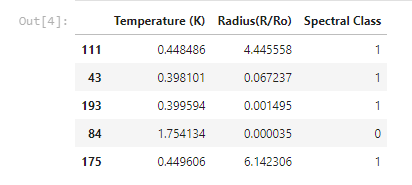
\includegraphics[width=10cm]{out1.png}
\label{figura:out1}
\end{figure}

Após isso, a regressão logística foi aplicada, a precisão da previsão foi avaliada e os pesos de influência de cada variável numérica foram calculados. A precisão desse modelo em específico foi de 1.0.
\\
\begin{lstlisting}
regressor = LogisticRegression(learning_rate=0.000001, n_iters=2000)
regressor.fit(X, y)
predictions = regressor.predict(X)

def accuracy(y_true, y_pred):
    accuracy = np.sum(y_true == y_pred) / len(y_true)
    return accuracy

print(f"A precisão do modelo é: {accuracy(y, predictions)}")

norma_pesos = pd.DataFrame(regressor.weights)/pd.DataFrame(regressor.weights).abs().sum()
norma_pesos = norma_pesos[0].values.tolist()

dfpesos = pd.DataFrame({'Pesos':norma_pesos}, index=dados['X'])

dfpesos
\end{lstlisting}

\begin{figure}[h]
\caption{Pesos de cada variável}
\centering
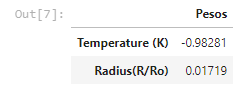
\includegraphics[width=10cm]{out2.png}
\label{figura:out2}
\end{figure}

\vspace{240px}

Por fim, foi feita uma visualização dessa regressão.
\\
\begin{lstlisting}
try:
    regressor.plot(X, y, dados['X'])
except:
    print("Sem visualização disponível.")
\end{lstlisting}

\begin{figure}[h]
\caption{Regressão linear - Resultado Final}
\centering
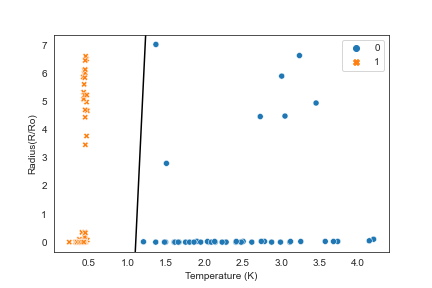
\includegraphics[width=10cm]{teste.png}
\label{figura:regressao_linear}
\end{figure}

\vspace{40px}
A partir disso, segue o resultado final obtido com as demais bases. 
\\
\begin{figure}[h]
\caption{Resultado final - vinhos}
\centering
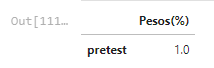
\includegraphics[width=10cm]{out4.png}
\label{figura:out4}
\end{figure}

\begin{figure}[h]
\caption{Resultado final - estudantes}
\centering
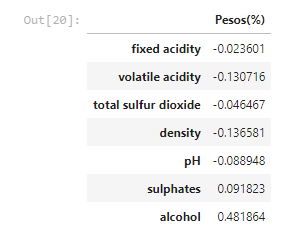
\includegraphics[width=10cm]{out3.png}
\label{figura:out3}
\end{figure}

\begin{figure}[h]
\caption{Resultado final - câncer de mama}
\centering
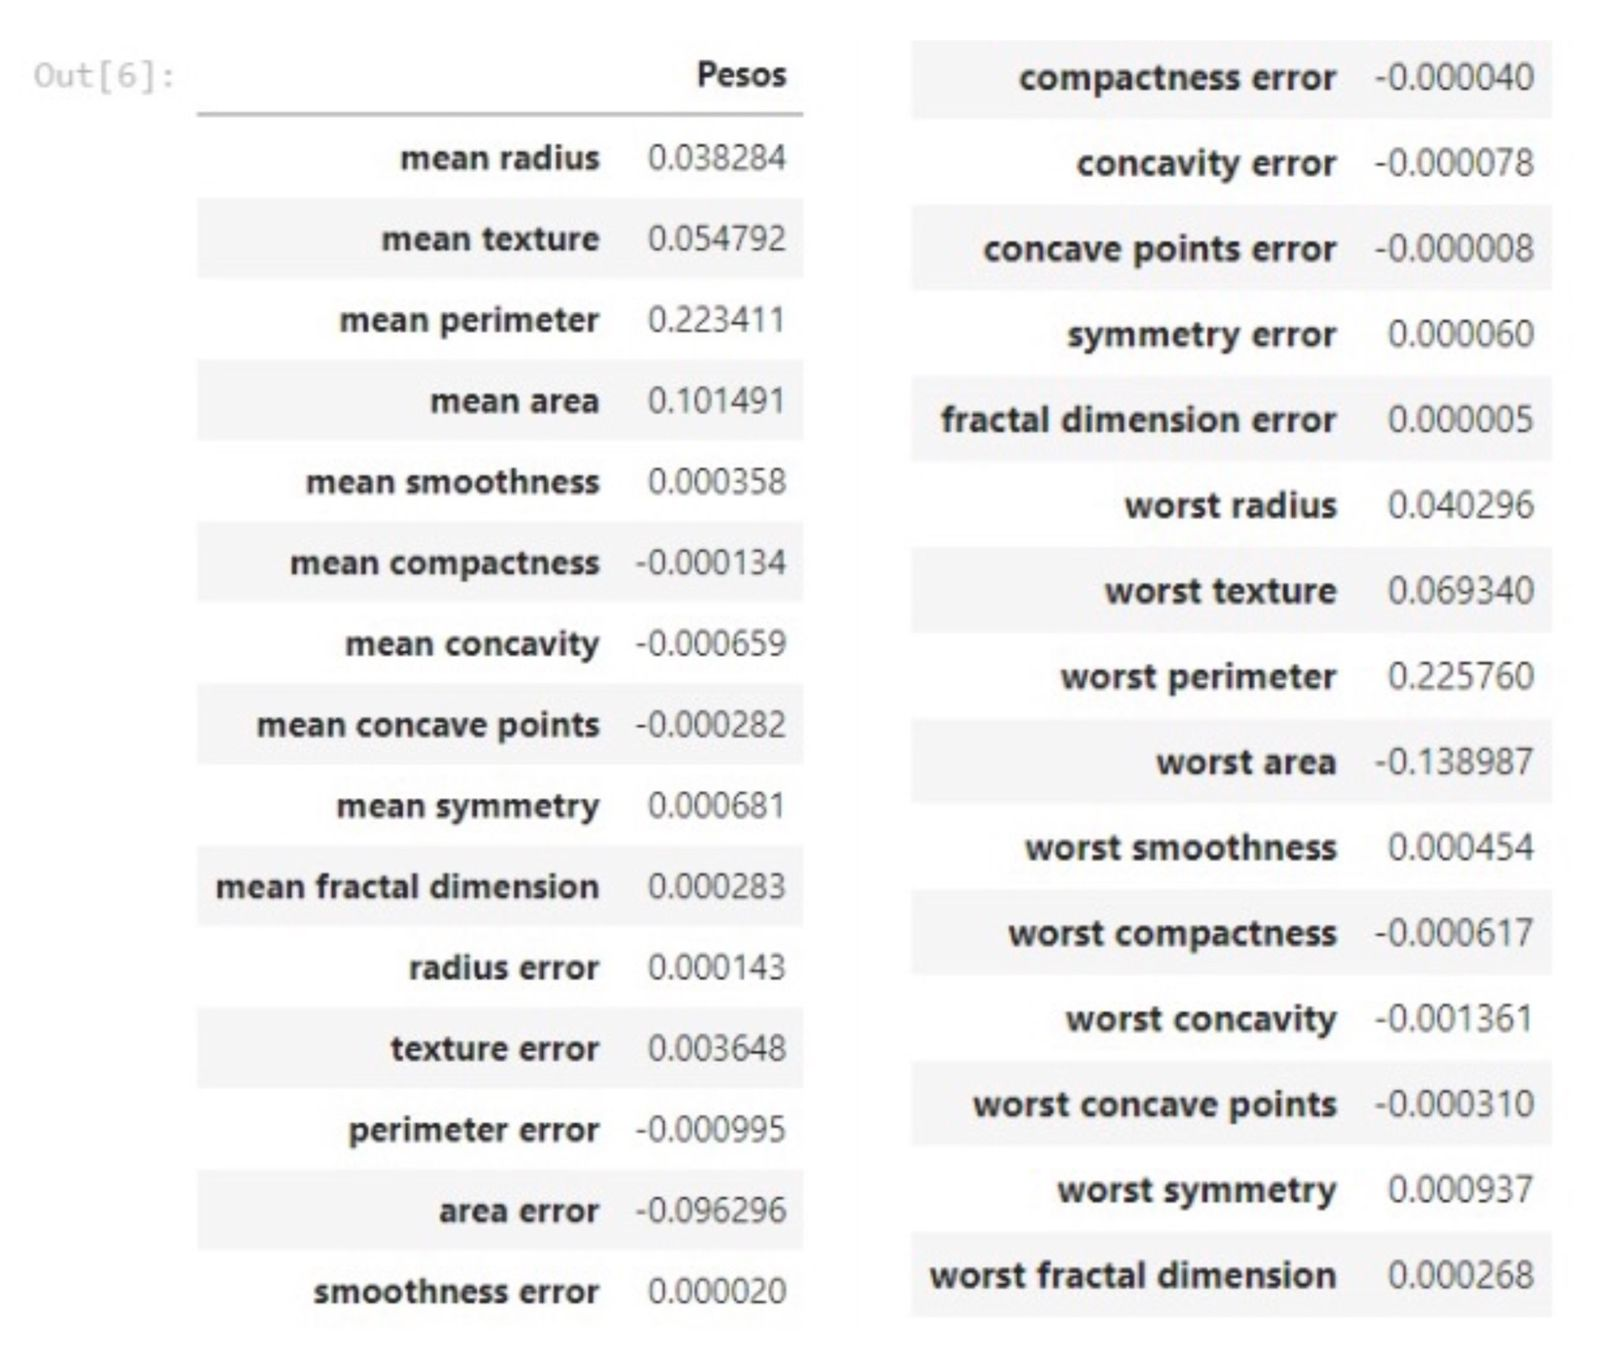
\includegraphics[width=10cm]{out5.jpeg}
\label{figura:out5}
\end{figure}

\clearpage
\section{Considerações Finais}

\hspace{0.4cm}Este trabalho se propôs, como objetivo geral, mostrar aplicações da regressão logística através de diferentes bases de dados. Desta forma, é possível concluir que é possível utilizar essa técnica em inúmeras áreas, onde ela sempre é destacada como uma importante ferramenta de análise de dados. 

\newpage
\section{Referências}

[1] a.\href{https://towardsdatascience.com/logistic-regression-from-scratch-with-numpy-da4cc3121ece}{ Towards Data Science - Logistic Regression from Scratch with NumPy}

\noindent [2] b.\href{https://monografias.ufma.br/jspui/bitstream/123456789/3572/1/LEANDRO-GONZALEZ.pdf}{ Leando Gonzales - Regressão Logística e suas aplicações}

\end{document}